\documentclass[12pt]{article}
\setlength\parindent{0pt}
\usepackage{fullpage}
\usepackage{amsmath}
\usepackage{graphicx}
\setlength{\parskip}{4mm}
\def\LL{\left\langle}   % left angle bracket
\def\RR{\right\rangle}  % right angle bracket
\def\LP{\left(}         % left parenthesis
\def\RP{\right)}        % right parenthesis
\def\LB{\left\{}        % left curly bracket
\def\RB{\right\}}       % right curly bracket
\def\PAR#1#2{ {{\partial #1}\over{\partial #2}} }
\def\PARTWO#1#2{ {{\partial^2 #1}\over{\partial #2}^2} }
\def\PARTWOMIX#1#2#3{ {{\partial^2 #1}\over{\partial #2 \partial #3}} }
\newcommand{\BE}{\begin{displaymath}}
\newcommand{\EE}{\end{displaymath}}
\newcommand{\BNE}{\begin{equation}}
\newcommand{\ENE}{\end{equation}}
\newcommand{\BEA}{\begin{eqnarray}}
\newcommand{\EEA}{\nonumber\end{eqnarray}}
\newcommand{\EL}{\nonumber\\}
\newcommand{\la}[1]{\label{#1}}
\newcommand{\ie}{{\em i.e.\ }}
\newcommand{\eg}{{\em e.\,g.\ }}
\newcommand{\cf}{cf.\ }
\newcommand{\etc}{etc.\ }
\newcommand{\Tr}{{\rm tr}}
\newcommand{\etal}{{\it et al.}}
\newcommand{\OL}[1]{\overline{#1}\ } % overline
\newcommand{\OLL}[1]{\overline{\overline{#1}}\ } % double overline
\newcommand{\OON}{\frac{1}{N}} % "one over N"
\newcommand{\OOX}[1]{\frac{1}{#1}} % "one over X"



\begin{document}
\Large
\centerline{\sc{Recitation Questions}}
\normalsize
\centerline{\sc{Week of April 10}}
\small

\medskip

\centerline{\large Question 0: torque and forces}

\centerline{(If you didn't finish this last week, finish it this week)}

 A unicyclist rides at a constant speed of 5 m/s; she and her unicycle have a combined mass of 70 kg. The wheel of her unicycle has a radius of 50 cm. At this speed, air resistance exerts a force of 80 N on her.

       1) What is the angular velocity of the wheel?
\vspace{1.2in}

       2) As you know, the force that wheeled vehicles use to propel themselves forward is static friction. What is the size of this force?
\vspace {1.2in}

       3) What torque must she apply to the wheel to maintain her speed?
\vspace{2in}

\newpage

       4) Suppose the pedals are attached to a crank with a radius of 25 cm. What force must she apply to the pedals to maintain her speed?
\vspace{3in}

       5) What power does she apply to the pedals? What power does the force of static friction apply to the unicycle? What power does the air resistance apply?

 \newpage

\centerline{\large Question 1: on static equilibrium}
\begin{minipage}[b]{0.4\textwidth}
  \vspace{-0.8in}

A 4m-long pole of mass 80 kg extends from the side of a building, angled at 60 degrees above the horizontal. One meter from the end of the pole, a sign of mass 50 kg is attached. To support the pole,
a horizontal cable runs from the end of the pole to the building. (See the attached figure.)

\bigskip
\bigskip
\bigskip
\bigskip
\bigskip
\bigskip

\end{minipage}
\begin{minipage}[t]{0.6\textwidth}
  \begin{flushright}
  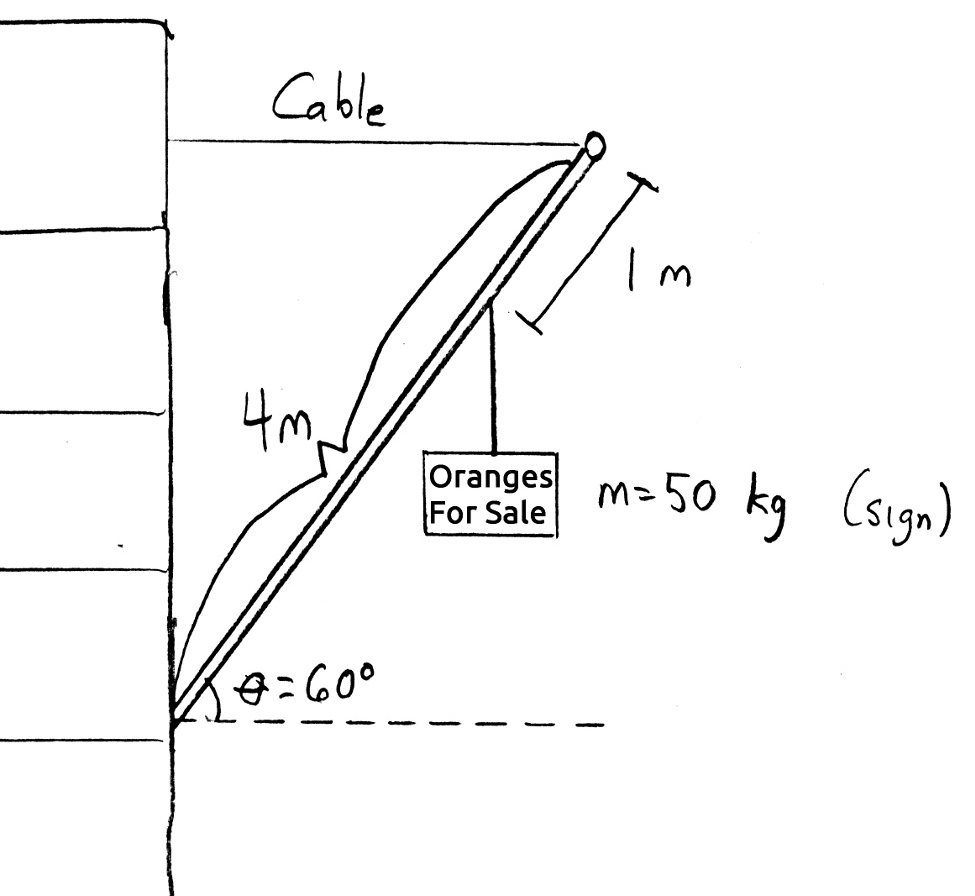
\includegraphics[width=0.9\textwidth]{sign2.jpg}
\end{flushright}
\end{minipage}

\bigskip
\bigskip


a) Draw a force diagram on the back of this page, showing all of the elements needed to help you compute the tension in the support cable. Indicate
your choice of pivot point.

\bigskip

b) Compute the tension in the cable. 

\vspace{2 in}

c) Suppose now that the store owner wanted to attach the cable to a different point on the building in order to minimize its tension. What angle between the
cable and the horizontal would support the pole with the minimum tension?
\newpage
\newpage
\rm
\centerline{\large Question 2: $F=ma$ and $\tau = I \alpha$ combined}
A Yo-Yo consists of a cylinder of mass $m$ and radius $r$. A slot is cut in the middle of the cylinder such that the inner radius is only $0.4r$, and a string is wound around the middle. (If you don't know what a Yo-Yo is, there is an animation on Wikipedia.)

\bigskip
\bigskip


A person holds the string and allows the Yo-Yo to fall. As it falls, it has both a linear acceleration (moving downward) and an angular acceleration (spinning faster and faster).

\begin{enumerate}

 \item{What is the relation between the linear velocity $v$ of the Yo-Yo (moving downward) and its angular velocity $\omega$?}

\vspace{1in}

       \item{What is the relation between the linear acceleration $a$ of the Yo-Yo (moving downward) and its angular velocity $\alpha$? (Note: this is trivial once you've done the previous part...)}

\vspace{1in}

       \item{Draw a force diagram for the Yo-Yo, indicating the location where all forces act as well as their magnitude.}
\vspace{3in}

       \item{Write down Newton's second law ($F=ma$) for the Yo-Yo, putting in expressions for the various forces.}

\vspace{2in}

       \item{Write down ``Newton's second law for rotation'' $\tau = I \alpha$, putting in expressions for the net torque and the moment of inertia.}

\vspace{2in}

       \item{What is the acceleration of the Yo-Yo and the tension in the string?}

\vspace{3in}

       \item{Will the Yo-Yo accelerate faster or slower if the inner radius is changed to $0.2r$?}

     \end{enumerate}





\end{document}
